\customHeader{1}{Preprocessing the \VSI{} dataset}
\label{vsi_preprocessing}

In response to the challenges outlined in \headerName{} \ref{vsi_data_issues}, we implemented multiple strategies.

% %%%%%%%%%%%%%%%%%%%%%%%%%%%%%%%%%%%%%%%%%%%%%%%%%%%%%%%%%%%%%%%%%%%%%%%%%%%%%%%%%%%%%%
\customHeader{2}{Leveraging Keywords}
\label{vsi_leveraging_keywords}

Leveraging the available keywords and key phrases used for the Google Search queries to construct the dataset (Table \ref{tab:04_query_keywords}), we obtained four more sources of content. 


We opted to extract sentences containing keywords or key phrases from the content. Using the Python package \texttt{NLTK} \myparencite{nltk}, we divided each document into phrases and selected those containing at least one of the keywords or key phrases. This process was carried out for both the \trafilaturaAbstract{} and \trafilaturaFulltext{} sources of content. However, considering the diverse range of languages in the documents, it was not always apparent whether we should discard the content entirely or retain it. For example, even if the keyword is not present in the text, maybe its translation is; or, the language could use a non-Latin script. Consequently, we pursued two different approaches: in one case, we discarded the original content (O.C.), and in the other, we retained it, resulting in four new sources of content:

\begin{itemize}
    \item \keyphrasesAbstractOnly{}
    \item \keyphrasesAbstractOC{}
    \item \keyphrasesFulltextOnly{}
    \item \keyphrasesFulltextOC{}
\end{itemize}


Figure \ref{fig:05_unique_entries_keyphrases_vsi} offers a comparison of the number of unique entries per content source. In both cases, keeping only the phrases containing keywords dramatically reduces the size of the data. Note that, in the case of keeping the original content, there are slightly less unique entries for both the \trafilaturaAbstract{} and the \trafilaturaFulltext{} ($19939-19798 = 141$ and $26346-24447=1899$, respectively). This may be explained by the fact that some data noise may be removed by the sentence extraction process, especially those cases where several entries differ by a small amount of tokens (see Table \ref{tab:04_website_names_as_suffixes}).

\begin{figure}
    \centering
    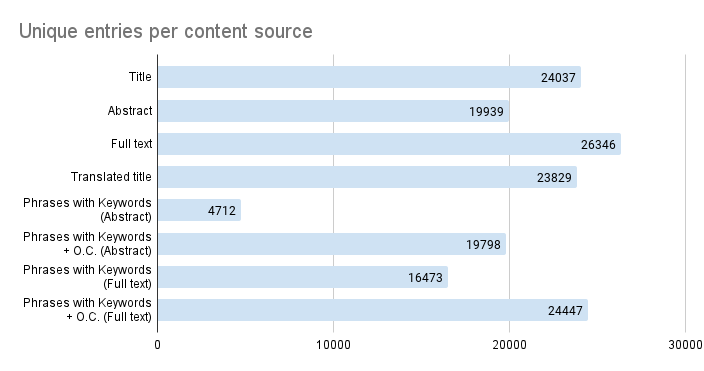
\includegraphics[width=0.750\textwidth]{Figures/05/Unique entries per content source_keyphrases.png}
    \caption{Unique entries per source of content in the \VSI{} dataset}
    \label{fig:05_unique_entries_keyphrases_vsi}
\end{figure}


% %%%%%%%%%%%%%%%%%%%%%%%%%%%%%%%%%%%%%%%%%%%%%%%%%%%%%%%%%%%%%%%%%%%%%%%%%%%%%%%%%%%%%%
\customHeader{2}{Data Cleaning}
\label{vsi_data_cleaning}


\customHeader{3}{Noise Removal}
\label{vsi_string_cleaning}

To address the text noise mentioned in \headerName{} \ref{vsi_issues_data_noise}, we use regular expressions to:

\begin{enumerate}
    \item Remove characters not in any human alphabet.
    \item Remove emojis, URLs, HTML tags, hours, dates, extra white spaces.
    \item Remove punctuation at beginning and end of the string.
    \item Remove digits at beginning and end of the string.
    \item Standardize quotation characters into the ASCII simple quotation character (').
    \item Standardize hyphen-like characters into the ASCII hyphen (-).
    \item Remove sentence suffixes that may be the name of the website, by deleting short text ($<=3$ tokens) that follow an ASCII hyphen near the end of the string.
\end{enumerate}

See Table \ref{appendix02:tab:pesv_string_cleaning_regex} in the \appendixname{} for some examples of the regular expressions used to clean the multilingual strings. Figure \ref{fig:05_multilingual_string_cleaning} shows the effect of string cleaning on an example text.

\begin{figure}
    \centering
    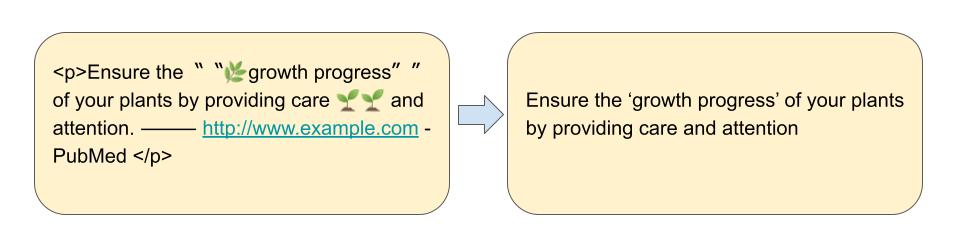
\includegraphics[width=\textwidth]{Figures/05/05_multilingual_string_cleaning.png}
    \caption{Removing noise from multilingual strings}
    \label{fig:05_multilingual_string_cleaning}
\end{figure}


\customHeader{3}{Deleting Error Messages}
\label{vsi_deleting_error_messages}

Fortunately, error messages in the dataset are very consistent. Given that they do not provide information on the relevance of a document, we may delete them using regular expressions. See Table \ref{appendix02:tab:error_messages} in the \appendixname{} for some examples of the regular expressions used to remove the error messages. 




\customHeader{3}{Handling scrapping errors}
% first attempt with title names regex. failed ~ 300 docs fewer
% second attempt: by length


In order to handle scraping errors from \trafilatura{}, such as obtaining the name of the website or certain HTML data headers, our first approach was using regular expressions to filter them out. After removing the error messages from all sources of content, we proceeded to count the occurrences of each entry and ranked them in descending order. Given that our dataset contains approximately 35,000 documents, we focused on entries that appeared at least twice.

Although we attempted to identify common patterns and create regular expressions to match frequent entries, this approach proved unsuccessful. It only filtered around 500 unique entries, accounting for a mere $2\%$ of all unique entries in the best case (\trafilaturaAbstract{}). Consequently, it became apparent that several scraping errors likely appeared only once in the dataset, rendering our previous strategy ineffective.

Nevertheless, along this examination, we noticed that scraping errors tend to be short in length (see Tables \ref{tab:04_headers} and \ref{tab:04_website_names}). As a result, we devised a new filtering strategy based on the length of the entries. However, simply counting naive tokens was insufficient, as languages like Chinese often lack whitespace in their text. Therefore, we needed a more robust algorithm to determine when a string is considered suspiciously ``too short."

Our algorithm to filter by length consists in:

\begin{enumerate}
    \item First, the string is split on white spaces.
    \item Then, if there is only one token, and the string has less than 20 characters, it is considered ``too short".
    \item Next, if there are less than four tokens, the string is considered ``too short"
    \item Finally, in all other cases, we keep the string.
\end{enumerate}


% %%%%%%%%%%%%%%%%%%%%%%%%%%%%%%%%%%%%%%%%%%%%%%%%%%%%%%%%%%%%%%%%%%%%%%%%%%%%%%%%%%%%%%
\customHeader{2}{Resolving Inconsistencies and Duplicate Documents}
\label{vsi_resolving_inconsistencies}





